\documentclass[12pt,a4paper]{extarticle}
\usepackage[utf8]{inputenc}
\usepackage[T5]{fontenc}
\usepackage{geometry}
\geometry{a4paper, left=1.5cm, right=1cm, top=1.5cm, bottom=1.5cm, headheight=20pt, headsep=15pt, footskip=28pt}
\usepackage{enumitem}
\usepackage{tikz}
\usetikzlibrary{patterns, patterns.meta} % Thêm patterns.meta vào đây
% Gọi package nằm trong thư mục con template
\usepackage{../template/mngocbox}

\begin{document}

% Sử dụng ngoặc vuông [...] để thay đổi linh hoạt các thông số
\makeheadbox[headerright={Tổng ôn 10-11},chude={CHỦ ĐỀ 02},tieude={Bất phương trình bậc nhất hai ẩn, hệ bất phương trình bậc nhất hai ẩn và Quy hoạch tuyến tính},dinhdang={Đại số},lop={12 },gv={Nguyễn Lê Minh Ngọc}]

\vspace{2em}
\makeheading{I}{Tóm tắt lý thuyết}
\section{Bất phương trình bậc nhất hai ẩn}
Bất phương trình bậc nhất hai ẩn $x, y$ có dạng tổng quát là \[ax + by \le c \quad (ax + by \ge c, \ ax + by < c, \ ax + by > c)\]
Trong đó $a, b, c$ là các số thực đã cho, $a$ và $b$ không đồng thời bằng $0$, $x$ và $y$ là các ẩn số.
\vspace{1cm}
Cặp số $(x_0, y_0)$ được gọi là \textbf{nghiệm} của bất phương trình bậc nhất hai ẩn $ax + by \le c$ nếu bất đẳng thức $ax_0 + by_0 \le c$ đúng.

\section{Biểu diễn miền nghiệm của bất phương trình bậc nhất hai ẩn}
Trong mặt phẳng tọa độ $Oxy$, tập hợp các điểm có tọa độ là nghiệm của bất phương trình được gọi là miền n
\paragraph{\textbf{\textit{Chú ý:}}} Nghiệm và miền nghiệm của các bất phương trình dạng $ax + by > c$, $ax + by \le c$ và $ax + by \ge c$ được định nghĩa tương tự.
Người ta chứng minh được rằng đường thẳng $d$ có phương trình $ax + by = c$ chia mặt phẳng tọa độ $Oxy$ thành hai nửa mặt phẳng bờ $d$:
\begin{itemize}
    \item Một nửa mặt phẳng (không kể bờ $d$) gồm các điểm có tọa độ $(x; y)$ thỏa mãn $ax + by > c$;
    \item Nửa mặt phẳng còn lại (không kể bờ $d$) gồm các điểm có tọa độ $(x; y)$ thỏa mãn $ax + by < c$.
\end{itemize}
Bờ $d$ gồm các điểm có tọa độ $(x; y)$ thỏa mãn $ax + by = c$.
\paragraph{\textbf{\textit{Chú ý:}}} Đối với bất phương trình dạng $ax + by \le c$ hoặc $ax + by \ge c$ thì miền nghiệm là nửa mặt phẳng kể cả đường thẳng $d$.

\paragraph{Biểu diễn miền nghiệm của bất phương trình bậc nhất hai ẩn}
Ví dụ với Các bước biểu diễn miền nghiệm của bất phương trình $ax + by < c$ trong mặt phẳng tọa độ $Oxy$ như sau:

\begin{center}
\renewcommand{\arraystretch}{2}
\begin{tabular}{|c|p{8.5cm}|c|}
\hline
\textbf{Thứ tự} & \hfil \textbf{Thực hiện} & \textbf{Đồ thị biểu diễn} \\ \hline
Bước 1 & Vẽ đường thẳng $d: ax + by = c$. Đường thẳng $d$ chia mặt phẳng tọa độ thành hai nửa mặt phẳng. & 
\begin{minipage}{5cm}
\centering
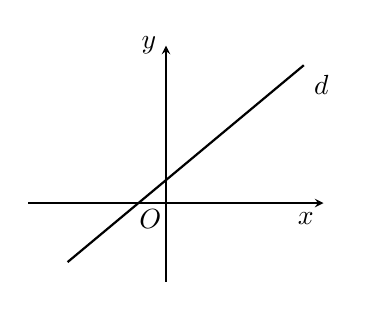
\begin{tikzpicture}[scale=0.5, >=stealth]
    \draw[->] (-3.5,0) -- (4,0) node[below left] {$x$};
    \draw[->] (0,-2) -- (0,4) node[left] {$y$};
    \draw (-0.4,-0.4) node {$O$};
    \draw[thick] (-2.5,-1.5) -- (3.5,3.5) node[below right] {$d$};
\end{tikzpicture}
\end{minipage} \\ \hline
Bước 2 & $\bullet$ Lấy một điểm $M(x_0; y_0)$ không nằm trên $d$ (thường lấy gốc tọa độ $O$ nếu $c \ne 0$) \newline
$\bullet$ Tính $ax_0 + by_0$ và so sánh với $c$ & 
\begin{minipage}{5cm}
~
\end{minipage} \\ \hline
Bước 3 & $\bullet$ Nếu $ax_0 + by_0 < c$ thì nửa mặt phẳng (không kể $d$) chứa điểm $M$ là miền nghiệm của bất phương trình $ax + by < c$. \newline (Phần gạch chéo không chứa $M$, tức là gạch phần nửa mặt phẳng bên dưới đường thẳng $d$). & 
\begin{minipage}{5cm}
\centering
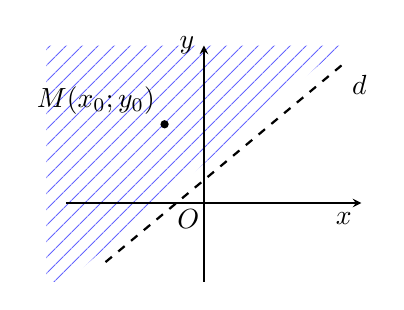
\begin{tikzpicture}[scale=0.5, >=stealth]
    \begin{scope}
        % Giới hạn vùng gạch chéo CHỈ ở nửa mặt phẳng BÊN DƯỚI đường thẳng d
        \clip (-3.5,-2) -- (3.5,4) -- (-4,4) -- (-4,-2) -- cycle;
        \fill[pattern={Lines[angle=45, distance={4pt}]}, pattern color=blue!60] (-5,-3) rectangle (5,5);
    \end{scope}
    \draw[->] (-3.5,0) -- (4,0) node[below left] {$x$};
    \draw[->] (0,-2) -- (0,4) node[left] {$y$};
    \draw (-0.4,-0.4) node {$O$};
    \draw[thick, dashed] (-2.5,-1.5) -- (3.5,3.5) node[below right] {$d$};
    \fill (-1,2) circle (3pt) node[above left] {$M(x_0;y_0)$};
\end{tikzpicture}
\end{minipage} \\ 
~ & $\bullet$ Nếu $ax_0 + by_0 > c$ thì nửa mặt phẳng (không kể $d$) không chứa điểm $M$ là miền nghiệm của bất phương trình $ax + by < c$. \newline (Phần gạch chéo chứa $M$, tức là gạch phần nửa mặt phẳng bên dưới đường thẳng $d$). & 
\begin{minipage}{5cm}
\centering
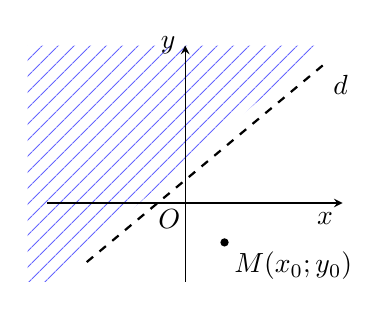
\begin{tikzpicture}[scale=0.5, >=stealth]
    \begin{scope}
        % Giới hạn vùng gạch chéo CHỈ ở nửa mặt phẳng BÊN DƯỚI đường thẳng d
        \clip (-3.5,-2) -- (3.5,4) -- (-4,4) -- (-4,-2) -- cycle;
        \fill[pattern={Lines[angle=45, distance={4pt}]}, pattern color=blue!60] (-5,-3) rectangle (5,5);
    \end{scope}
    \draw[->] (-3.5,0) -- (4,0) node[below left] {$x$};
    \draw[->] (0,-2) -- (0,4) node[left] {$y$};
    \draw (-0.4,-0.4) node {$O$};
    \draw[thick, dashed] (-2.5,-1.5) -- (3.5,3.5) node[below right] {$d$};
    
    % Điểm M(-1,3) nằm hoàn toàn bên phần TRẮNG (không gạch chéo)
    \fill (1,-1) circle (3pt) node[below right] {$M(x_0;y_0)$};
\end{tikzpicture}
\end{minipage} \\ \hline
\end{tabular}
\end{center}

\paragraph{\textbf{\textit{Chú ý:}}} Thông thường khi sử dụng phần mềm toán học để biểu diễn miền nghiệm của bất phương trình bậc nhất hai ẩn, miền nghiệm của bất phương trình đó được tô màu.
\section{Biểu diễn miền nghiệm của hệ bất phương trình bậc nhất hai ẩn}
\paragraph{Biểu diễn miền nghiệm của hệ bất phương trình sau:} 
$\begin{cases}
    a_1x + b_1y > c_1 \\
    a_2x + b_2y > c_2 \\
    a_3x + b_3y < c_3
\end{cases}$

\begin{center}
\renewcommand{\arraystretch}{2}
\begin{tabular}{|c|p{8.5cm}|c|}
\hline
\textbf{Thứ tự} & \hfil \textbf{Thực hiện} & \textbf{Đồ thị biểu diễn} \\ \hline
Bước 1 & Vẽ các đường thẳng
\begin{itemize}
    \item $d_1: a_1x + b_1y = c_1$
    \item $d_2: a_2x + b_2y = c_2$
    \item $d_3: a_3x + b_3y = c_3$
\end{itemize} & 
\begin{minipage}{5cm}
\centering
\vspace{0.5em}
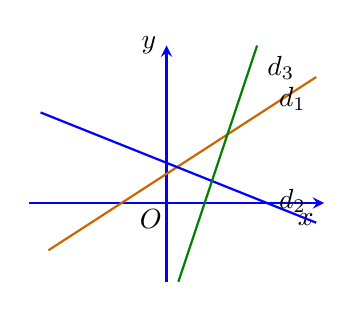
\begin{tikzpicture}[scale=0.5, >=stealth]
    % Trục tọa độ
    \draw[->, color=blue, thick] (-3.5,0) -- (4,0) node[below left, color=black] {$x$};
    \draw[->, color=blue, thick] (0,-2) -- (0,4) node[left, color=black] {$y$};
    \draw (-0.4,-0.4) node {$O$};
    
    % Vẽ các đường thẳng d1, d2, d3
    \draw[thick, color=orange!80!black] (-3,-1.2) -- (3.8,3.2) node[below left, color=black] {$d_1$};
    \draw[thick, color=blue] (-3.2,2.3) -- (3.8,-0.5) node[above left, color=black] {$d_2$};
    \draw[thick, color=green!50!black] (0.3,-2) -- (2.3,4) node[below right, color=black] {$d_3$};
\end{tikzpicture}
\vspace{0.5em}
\end{minipage} \\ \hline
Bước 2 & Biểu diễn miền nghiệm của các bất phương trình, bằng cách gạch bỏ phần không thuộc miền nghiệm của nó.
\begin{itemize}
    \item $a_1x + b_1y > c_1$
    \item $a_2x + b_2y > c_2$
    \item $a_3x + b_3y < c_3$
\end{itemize}
Phần không bị gạch là miền nghiệm cần tìm. & 
\begin{minipage}{5cm}
\centering
\vspace{0.5em}
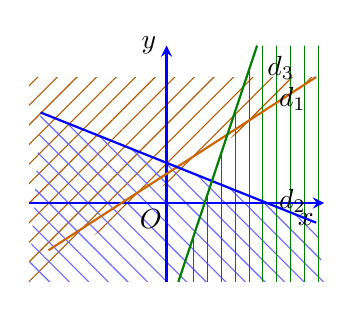
\begin{tikzpicture}[scale=0.5, >=stealth]
    \begin{scope}
        % Gạch chéo của d1 (phần phía dưới d1)
        \clip (-3.5,-2) rectangle (4,4);
        \clip (-3.5,-2) -- (3.8,3.2) -- (-3.5,3.2) -- cycle;
        \fill[pattern={Lines[angle=45, distance={5pt}]}, pattern color=orange!70!black] (-4,-3) rectangle (5,5);
    \end{scope}
    
    \begin{scope}
        % Gạch chéo của d2 (phần phía dưới d2)
        \clip (-3.5,-2) rectangle (4,4);
        \clip (-3.5,-2) -- (-3.2,2.3) -- (3.8,-0.5) -- (4,-2) -- cycle;
        \fill[pattern={Lines[angle=-45, distance={5pt}]}, pattern color=blue!60] (-4,-3) rectangle (5,5);
    \end{scope}
    
    \begin{scope}
        % Gạch chéo của d3 (phần bên phải d3)
        \clip (-3.5,-2) rectangle (4,4);
        \clip (0.3,-2) -- (2.3,4) -- (4,4) -- (4,-2) -- cycle;
        \fill[pattern={Lines[angle=90, distance={5pt}]}, pattern color=green!50!black] (-4,-3) rectangle (5,5);
    \end{scope}

    % Vẽ lại hệ trục tọa độ đè lên phần gạch
    \draw[->, color=blue, thick] (-3.5,0) -- (4,0) node[below left, color=black] {$x$};
    \draw[->, color=blue, thick] (0,-2) -- (0,4) node[left, color=black] {$y$};
    \draw (-0.4,-0.4) node {$O$};
    
    % Vẽ lại các đường thẳng (nét đứt hoặc nét liền tùy ý, ở đây giữ nguyên nét liền như ảnh)
    \draw[thick, color=orange!80!black] (-3,-1.2) -- (3.8,3.2) node[below left, color=black] {$d_1$};
    \draw[thick, color=blue] (-3.2,2.3) -- (3.8,-0.5) node[above left, color=black] {$d_2$};
    \draw[thick, color=green!50!black] (0.3,-2) -- (2.3,4) node[below right, color=black] {$d_3$};
\end{tikzpicture}
\vspace{0.5em}
\end{minipage} \\ \hline
\end{tabular}
\end{center}
\makeheading{II}{Bài tập tự luyện}
\textbf{1.} Một cửa hàng dành tối đa 10 triệu để nhập $x$ tạ gạo và $y$ tạ mì. Biết mỗi tạ gạo mua hết 1,5 triệu, mỗi tạ mì mua hết 1,2 triệu. Khi đó:
\begin{itemize}
    \item[a)] Bất phương trình biểu thị mối liên hệ giữa $x$ và $y$ là: $1,5x + 1,2y \le 10$.
    \item[b)] Bất phương trình biểu thị mối liên hệ giữa $x$ và $y$ là: $1,5x + 1,2y \ge 10$.
    \item[c)] Miền nghiệm của bất phương trình $1,5x + 1,2y \le 10$ là nửa mặt phẳng bờ là đường thẳng $1,5x + 1,2y = 10$ chứa điểm $O(0; 0)$.
    \item[d)] Miền nghiệm của bất phương trình $1,5x + 1,2y \le 10$ là nửa mặt phẳng bờ là đường thẳng $1,5x + 1,2y = 10$ không chứa điểm $O(0; 0)$.
\end{itemize}

\textbf{2.} Ông An muốn thuê một chiếc ô tô (có lái xe) trong một tuần. Giá thuê xe được cho như bảng sau:

\begin{center}
\begin{tabular}{|l|c|c|}
\hline
 & \textbf{Phí cố định} & \textbf{Phí tính theo quãng đường di chuyển} \\
 & (nghìn đồng/ngày) & (nghìn đồng/kilômét) \\
\hline
Từ thứ Hai đến thứ Bảy & 800 & 10 \\
\hline
Chủ nhật & 1200 & 15 \\
\hline
\end{tabular}
\end{center}

Gọi $x$ và $y$ lần lượt là số kilômét ông An đi trong các ngày từ thứ Hai đến thứ Bảy và trong Chủ nhật. Khi đó các mệnh đề sau đúng hay sai?
\begin{itemize}
    \item[a)] Số tiền ông An phải trả khi thuê xe từ thứ Hai đến thứ Bảy là $10x$ (nghìn đồng).
    \item[b)] Số tiền ông An phải trả khi thuê xe trong Chủ nhật là $1200 + 15y$ (nghìn đồng).
    \item[c)] Bất phương trình biểu thị mối liên hệ giữa $x$ và $y$ sao cho tổng số tiền ông An phải trả không quá 16 triệu đồng là $2x + 3y < 2000$.
    \item[d)] Miền nghiệm của bất phương trình biểu thị mối liên hệ giữa $x$ và $y$ sao cho tổng số tiền ông An phải trả không quá 16 triệu đồng là nửa mặt phẳng phần không bị tô đậm trong hình bên dưới có bờ là đường thẳng $d: 2x + 3y = 2000$ (lấy cả những điểm nằm trên đường thẳng $d: 2x + 3y = 2000$).
\end{itemize}
\begin{center}
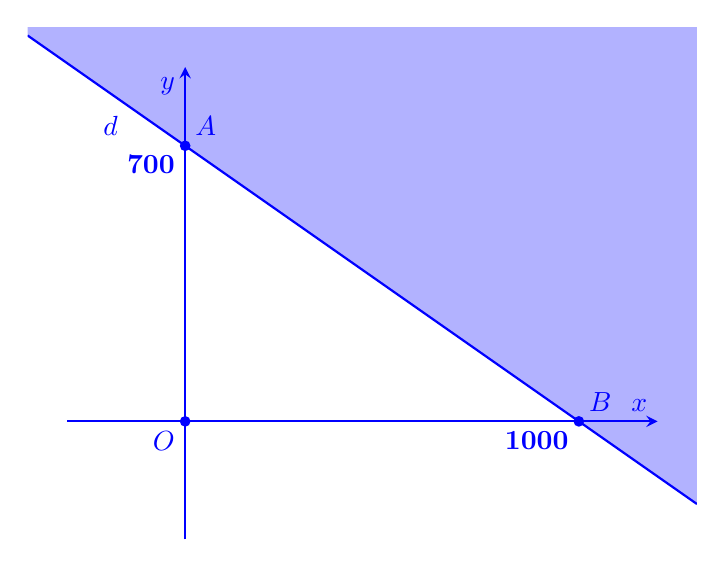
\begin{tikzpicture}[>=stealth, thick, color=blue]
    
    % Giới hạn vùng vẽ
    \clip (-2, -1.5) rectangle (6.5, 5);

    % Tô màu miền nghiệm (vùng màu hồng nhạt)
    % Đường thẳng d có phương trình y = -0.7x + 3.5
    % Điểm đầu (-3, 5.6), Điểm cuối (8, -2.1)
    \fill[blue!30] (-3, 5.6) -- (8, -2.1) -- (8, 6) -- cycle;

    % Vẽ các trục tọa độ
    \draw[->] (-1.5, 0) -- (6, 0) node[above left] {$x$};
    \draw[->] (0, -1.5) -- (0, 4.5) node[below left] {$y$};

    % Vẽ đường thẳng d
    \draw (-2, 4.9) -- (6.5, -1.05) node[pos=0.15, below left] {$d$};

    % Vẽ các điểm và nhãn
    % Gốc tọa độ O
    \filldraw (0,0) circle (1.5pt) node[below left] {$O$};
    
    % Điểm A(0, 700) - Thu nhỏ tỷ lệ 1/200 thành (0, 3.5)
    \filldraw (0, 3.5) circle (1.5pt) node[above right] {$A$} node[below left] {$\mathbf{700}$};
    
    % Điểm B(1000, 0) - Thu nhỏ tỷ lệ 1/200 thành (5, 0)
    \filldraw (5, 0) circle (1.5pt) node[above right] {$B$} node[below left] {$\mathbf{1000}$};

\end{tikzpicture}
\end{center}
\textbf{3.} Bạn Lan có $15$ nghìn đồng để đi mua vở. Vở loại $A$ có giá $3000$ đồng một cuốn, vở loại $B$ có giá $4000$ đồng một cuốn. Hỏi bạn Lan có thể mua nhiều nhất bao nhiêu quyển vở sao cho bạn có cả hai loại vở?\\
\vspace{1cm}

\textbf{4.} Trong $1$ lạng ($100\text{ g}$) thịt bò chứa khoảng $26\text{ g}$ protein, $1$ lạng cá rô phi chứa khoảng $20\text{ g}$ protein. Trung bình trong một ngày, một người phụ nữ cần tối thiểu $46\text{ g}$ protein. (\textit{Nguồn: \url{https://vinmec.com} và \url{https://thanhnien.vn}}) Gọi $x, y$ lần lượt là số lạng thịt bò và số lạng cá rô phi mà một người phụ nữ nên ăn trong một ngày. Viết bất phương trình bậc nhất hai ẩn $x, y$ để biểu diễn lượng protein cần thiết cho một người phụ nữ trong một ngày và chỉ ra ba nghiệm của bất phương trình đó.\\
\vspace{1cm}

\textbf{5.} Bạn Nga muốn pha hai loại nước rửa xe. Để pha một lít loại I cần 600ml dung dịch chất tẩy rửa, còn loại II cần 400ml. Gọi x và y lần lượt là số lít nước rửa xe loại I và II và biết rằng bạ chỉ còn 2400ml chất tẩy rửa, hãy lập các bất phương trình mô tả số lít nước rửa xe loại I và II mà bạn đó có thể pha chế được và biểu diễn miền nghiệm của từng bất phương trình đó trên mặt phẳng toạ độ Oxy.
\end{document}